\documentclass[aspectratio=1610]{ctexbeamer}
\usetheme{Berlin}
\usepackage{xeCJK}
\usepackage{multirow}
\usepackage{graphicx}
\usepackage{booktabs} % for better table formatting
\usepackage{geometry} % for adjusting page layout
% \usepackage{enumitem} % for customizing lists
\usepackage{hyperref} % for clickable links and references
\usepackage{subcaption}
\usepackage{tikz}
\usepackage{amsmath}
\usepackage{colortbl}
\newcommand\DiagonalCell[2]{%
  \begin{tikzpicture}[baseline=(current bounding box.center),anchor=center]
    \node[minimum width=0.8cm,minimum height=2em] (box) {};
    \draw (box.north west) -- (box.south east);
    \node[anchor=south west,inner sep=1pt,outer sep=0pt] at (box.south west) {#1};
    \node[anchor=north east,inner sep=1pt,outer sep=0pt] at (box.north east) {#2};
  \end{tikzpicture}%
}
\usepackage{xcolor}
\usetikzlibrary{quantikz}
\setbeamertemplate{itemize item}[ball] % Can be circle, square, etc.
\setbeamertemplate{itemize subitem}[default] % Can be ball, triangle, etc.
\title[学位论文答辩]{基于TDD的量子模型检测中的可达性分析}
\subtitle{硕士学位论文答辩}
\author[Gc]{高丁超\\ 导师:应圣钢}
\institute[ISCAS]{中国科学院软件研究所}
\AtBeginSection[]{
  \ifthenelse{\equal{\secname}{End}}{}{ % Checks if the section name is "End"
    \begin{frame}<beamer> % Only creates the frame if the section is not "End"
        \frametitle{目录}
        \tableofcontents[currentsection]
    \end{frame}
  }
}

\begin{document}
\begin{frame}[plain]
    \titlepage
    \begin{figure}
        \centering
        \begin{subfigure}[c]{0.4\textwidth}
            \centering
            \includegraphics[height= 2cm]{Img/iscas.png}
        \end{subfigure}
        \qquad
        \begin{subfigure}[c]{0.4\textwidth}
            \centering
            \includegraphics[height= 2cm]{Img/ucas.jpg}
        \end{subfigure}
    \end{figure}
    %  Title page
\end{frame}
\begin{frame}
    \frametitle{目录}
    \tableofcontents
\end{frame}

\section{背景介绍}

\begin{frame}
    \begin{itemize}
        \item \textbf{标题:} 基于张量网络的量子模型检测中的可达性分析
        \item \textbf{总结:}
        \begin{itemize}
            \setlength\itemsep{1em} % Set item separation here, for subitems
            \item \textit{问题:} 如何在量子系统中验证命题。
            \item \textit{解决方案:} 采用量子模型检测。
            \item \textit{挑战:} 原有的方法随着量子比特数量的增加,资源需求指数级增长。
            \item \textit{方法:} 引入新的数据结构TDD对量子算法进行表示,同时实现了优化算法进一步减少了时间消耗。
        \end{itemize}
    \end{itemize}
\end{frame}

\begin{frame}{量子计算的关键概念}
    \begin{itemize}
        \item \textbf{量子比特(Qubits):} the quantum version of the classic binary
        \item \textbf{叠加态(Superposition):} $|\psi\rangle = \alpha |0\rangle + \beta |1\rangle=\left[\begin{array}{r}\alpha \\\beta\end{array}\right]$
        \item \textbf{纠缠(Entanglement):}$|\Psi\rangle = \frac{1}{\sqrt{2}}(|00\rangle+|11\rangle)$
        \item \textbf{量子门(Quantum Gates)} 
    \end{itemize}
\end{frame}
\begin{frame}{量子门操作例子}
    \begin{itemize}
        \item \textbf{单量子门例子:}$X=\left[\begin{array}{rr}0 & 1 \\1 & 0 \end{array}\right],Y=\left[\begin{array}{rr}0 & -i \\i & 0 \end{array}\right],Z=\left[\begin{array}{rr}1 & 0 \\0 & -1 \end{array}\right],H=\frac{1}{\sqrt{2}}\left[\begin{array}{rr}1 & 1 \\1 & -1 \end{array}\right]$ 
        \item \textbf{多量子门例子:} $\text { CNOT }=\left[\begin{array}{llll}
            1 & 0 & 0 & 0 \\
            0 & 1 & 0 & 0 \\
            0 & 0 & 0 & 1 \\
            0 & 0 & 1 & 0
            \end{array}\right]$
        \item \textbf{测量,比如$Z$基测量:}状态为$|0\rangle$输出$1$,状态为$|1\rangle$输出$-1$。
    \end{itemize}
\end{frame}
\begin{frame}{量子计算例子}
    \begin{figure}[h]
      \centering
      \scalebox{1.1}{
      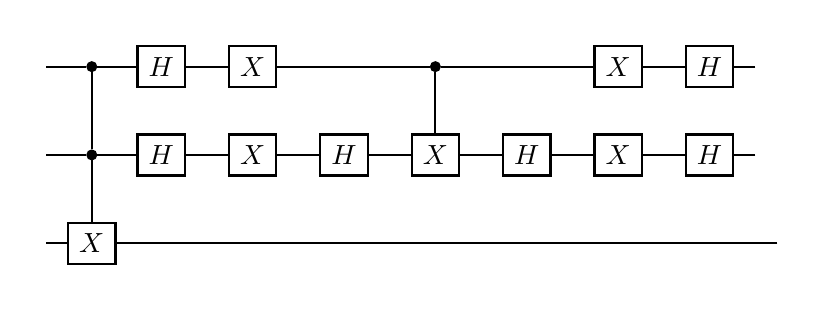
\begin{tikzpicture}
      \node at (0,0) [anchor=north]{
      \begin{quantikz}[column sep=0.28cm,row sep=0.6cm]
      &\ctrl{1}&\gate{H}&\qw&\gate{X}&\qw&\qw&\qw     &\ctrl{1}&\qw&\qw&\qw     &\gate{X}&\qw&\gate{H}&\qw \\
      &\ctrl{1}&\gate{H}&\qw&\gate{X}&\qw&\gate{H}&\qw&\gate{X}&\qw&\gate{H}&\qw&\gate{X}&\qw&\gate{H}&\qw \\
      &\gate{X}&\qw     &\qw     &\qw     &\qw     &\qw     &\qw     &\qw     &\qw&\qw&\qw&\qw&\qw&\qw&\qw&\qw 
      \end{quantikz}};
      \end{tikzpicture}
      }
      \label{fig:cir}
      \caption{Grover\_3算法的电路。}
    \end{figure}
\end{frame}
\begin{frame}{研究背景}
    \begin{itemize}
        \item<1-> 量子计算的快速发展
        \begin{itemize}
            \item 规模化拓展
            \begin{itemize}
                \item IBM: Condor \textbf{1121}; 中科大: 九章三号 \textbf{255}
            \end{itemize}
            \item 容错计算
            \begin{itemize}
                \item IonQ: \textbf{29}; QuEra:  \textbf{48}
            \end{itemize}
        \end{itemize}
        \item<2-> 现有验证方法
        \begin{itemize}
            \item 模型检测自动化程度高,但存在资源爆炸的问题
            \item 定理证明处理复杂问题有明显优势,但自动化程度低
        \end{itemize}
    \end{itemize}
\end{frame}
\begin{frame}{量子迁移系统}
    \begin{columns}[T] % The "T" option aligns the columns content at the top

        % Column for itemized list
        \begin{column}{.6\textwidth}
            \begin{itemize}
                \item  \textbf{迁移系统(transition system):} $(S, I, \Sigma, T)$
                \begin{equation}
                  where
                  \begin{cases}
                    x = x_1, \cdots, x_n\\
                    y = y_1, \cdots, y_n\\
                    \sigma = \sigma_1, \cdots, \sigma_m
                  \end{cases}
                  \notag
                \end{equation}
                \item \textbf{量子迁移系统:} $(\mathcal{H},S,\Sigma,\mathcal{T})$
            \end{itemize}
        \end{column}
    
        % Column for figure
        \begin{column}{.3\textwidth}
          \begin{figure}
            \centering
            \includegraphics[width=\textwidth]{Img/transition.png}
          \end{figure}
        \end{column}
    
      \end{columns}
\end{frame}
\begin{frame}{可达性问题}
    \begin{figure}
        \includegraphics[width=.6\textwidth]{Img/eventually.png}
    \end{figure}
    \begin{figure}
        \includegraphics[width=.6\textwidth]{Img/eventuallyalways.png}
    \end{figure}
    \begin{figure}
        \includegraphics[width=.6\textwidth]{Img/alwayseventually.png}
    \end{figure}
  \end{frame}
%   \begin{frame}{量子逻辑}
%     \begin{itemize}[itemsep=18pt]
%         \item \textbf{子集关系 \( \subseteq \) 在 \(S(\mathcal{H})\) 中:} 偏序关系,表示蕴涵。
%         \item \textbf{正交补 \( \mathcal{X}^\perp \):} 表示否定。
%         \item \textbf{闭合于交集:} \( \bigcap_{i} \mathcal{X}_{i} \in S(\mathcal{H}) \),表示合取。
%         \item \textbf{子空间的并集:} \( \bigvee_i \mathcal{X}_i = \text{span} \left( \bigcup_i \mathcal{X}_i \right) \),解释为析取。
%     \end{itemize}
% \end{frame}

\begin{frame}{量子模型检测例子}
    \begin{figure}[h]
        \centering
        \scalebox{0.8}{
        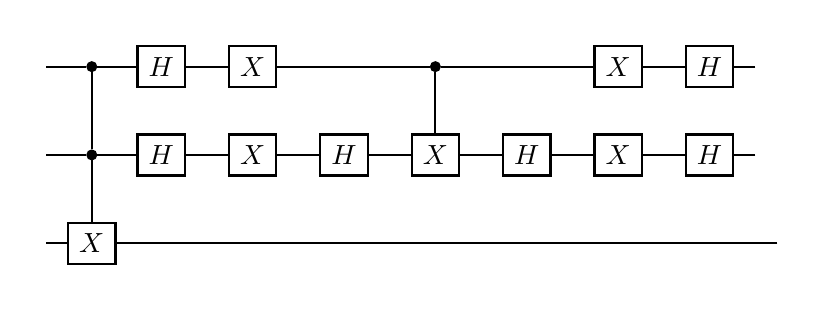
\begin{tikzpicture}
        \node at (0,0) [anchor=north]{
        \begin{quantikz}[column sep=0.28cm,row sep=0.6cm]
        &\ctrl{1}&\gate{H}&\qw&\gate{X}&\qw&\qw&\qw     &\ctrl{1}&\qw&\qw&\qw     &\gate{X}&\qw&\gate{H}&\qw \\
        &\ctrl{1}&\gate{H}&\qw&\gate{X}&\qw&\gate{H}&\qw&\gate{X}&\qw&\gate{H}&\qw&\gate{X}&\qw&\gate{H}&\qw \\
        &\gate{X}&\qw     &\qw     &\qw     &\qw     &\qw     &\qw     &\qw     &\qw&\qw&\qw&\qw&\qw&\qw&\qw&\qw 
        \end{quantikz}};
        \end{tikzpicture}
        }
        \caption{Grover\_3算法的电路。}
        \label{fig:cir}
    \end{figure}
    \begin{itemize}
        \item oracle为ccx,即$O|x\rangle|y\rangle = |x\rangle|f(x)\oplus y\rangle $,$f(x)=x_1\wedge x_2$。
        \item \textbf{model:} $(\mathcal{H}_8, S = span\{|++-\rangle,|11-\rangle\}, \{1\}, {\mathcal{T}_1})$, $\mathcal{T}_1 =(2|\Psi\rangle\langle \Psi| - I)O$ 
        \item \textbf{property:} $\mathcal{T}_1(S)=S$
    \end{itemize}
\end{frame}

% \begin{frame}{量子模型检测例子}
%     \begin{figure}
%       \includegraphics[height=3.5cm]{Img/cir_coum.pdf}
%       \caption{一个量子通信协议例子,其中$|\Psi\rangle = \frac{1}{\sqrt{2}}(|00\rangle+|11\rangle)$}
%     \end{figure}
% \end{frame}
% \begin{frame}{量子模型检测例子}
%     \begin{figure}
%         \centering
%         \begin{subfigure}{0.3\textwidth}
%           \includegraphics[width=\textwidth]{Img/rus_s.pdf}
%         \end{subfigure}
%         \quad
%         \begin{subfigure}{0.3\textwidth}
%           \includegraphics[width=\textwidth]{Img/rus_T.pdf}
%         \end{subfigure}
%         \caption{两个rus电路}
%     \end{figure}
% \end{frame}
\begin{frame}{张量决策图(TDD)}
    \begin{itemize}
        \item \textbf{TDD 定义:} 由节点集 $V$、边集 $E$、索引函数 $index$、值函数 $value$、低高边映射 $low/high$ 和权重 $w$ 组成。
        \item
        \begin{itemize}
            \item 节点集$V$分为非终端节点 $V_N$ 和终端节点 $V_T$,且有唯一根节点 $r_{\mathcal{F}}$。
            \item 边集$E$包含所有低边 $\left(v,low(v)\right)$ 和高边 $\left(v,high(v)\right)$。
            \item 索引函数$index$ 分配索引,值函数$value$ 赋予终端节点复数值,$w$ 为边赋权重,特别是根边权重 $w_{\mathcal{F}}$。
        \end{itemize}
    \end{itemize}
\end{frame}

\begin{frame}{TDD例子}
    \begin{figure}
        \begin{subfigure}{0.4\textwidth}
            \includegraphics[height=3.5 cm]{Img/matrix_of_tdd.pdf}
            \label{fig:mat_P}
        \end{subfigure}
        \qquad
        \qquad
        \qquad
        \begin{subfigure}[c]{0.4\textwidth}
            \centering
            \includegraphics[height=6cm]{Img/tdd_ex.pdf}
            \label{fig:tdd_P}
        \end{subfigure}
        \label{fig:P}
        \caption{可以用10个TDD节点或者一个$8*8$的矩阵表示子空间$S=span\{\ket{++-},\ket{11-}\}$投影算子。其中TDD虚线表示低点,实线表示高边。}
    \end{figure}
\end{frame}
% \begin{frame}{相关工作效率比较}
%     \begin{figure}
%         \includegraphics[height=4cm]{Img/tdd-compare.pdf}
%         \caption{应用不同技术对QFT算法进行模拟的时间对比}
%     \end{figure}
%     \begin{center}
%         \begin{itemize}
        
%             \item TDD No part,TDD part I, TDD part II为不同的TDD收缩算法。 
%             \item QMDD为量子多值决策图,是一种常用的模型检测方法。
%             \item TN为Google的tensro network,是一种常用的张量方法。
%         \end{itemize}
%     \end{center}
% \end{frame}
% \begin{frame}{相关工作-QMDD}
%     \begin{columns}[T] % The "T" option aligns the columns content at the top

%         % Column for itemized list
%         \begin{column}{.6\textwidth}
%             \begin{figure}
%                 \includegraphics[height=4cm]{Img/QMDD_b.png}
%                 \caption{一个QMDD的示例。}
%             \end{figure}
%         \end{column}
%         \begin{column}{.4\textwidth}
%             \hspace{80pt}
%             \begin{itemize}
%                 \item TDD只有高边和低边,表示更简洁。
%             \end{itemize}
%         \end{column}
        
%     \end{columns}
%   \end{frame}
\section{研究内容}
\begin{frame}{解决方案简介:}
    \begin{itemize}
        \item \textbf{研究问题:}减缓量子模型检测中的资源消耗
        \item \textbf{基本方法:}将转移关系和状态空间转化为TDD表示,然后计算系统的状态转移。
        \item \textbf{改进算法:}
        \begin{itemize}
            \item \textbf{addition partition:} 寻找依赖最多的索引项,从而分割线路。
            \item \textbf{contraction partition:}通过预设的参数进行线路分割。
        \end{itemize}
        \begin{itemize}
            \item \textbf{基于窗函数对TDD分割:}
            \item \textbf{用子空间近似TDD表示$\ket{\psi}$}
        \end{itemize}
        % \item \textbf{创新点:}
        % % \item //TODO: add new
        % \begin{itemize}
        %     \item 通过TDD,可以自动化的验证更大规模的量子算法。
        %     \item 
        %     % \item 通过C++重构,实现了比过去TDD更好的运行效率。
        % \end{itemize}
    \end{itemize}
\end{frame}
% //TODO: add some alg
\begin{frame}{理论支撑}
    对于$(\mathcal{H},S,\Sigma,\mathcal{T})$有:
    \begin{theorem}
        \label{theorem-model}
        设 $\mathcal{T}$ 是一个量子操作。则
    \begin{enumerate}
        \item $\mathcal{T}(\bigvee_{i}{S_i})=\bigvee_{i}{\mathcal{T}(S_i)}$。
        \item 若 $\mathcal{T}=(\mathcal{T}_\sigma)_{\sigma \in \Sigma}$ 且每个 $\mathcal{T}_{\sigma}$ 有Kraus算符和表示 $\mathcal{T}_{\sigma}= \{ E_{\sigma j_\sigma} \}$
    则
    $\mathcal{T}(S)=span\Big(\bigcup_{\sigma,j_\sigma}{\{E_{\sigma j_\sigma}\ket{\psi}:\ket{\psi}\in S\}}\Big)$。
    \end{enumerate}
    \end{theorem}
\end{frame}
\begin{frame}{子空间}
    \begin{columns} % The "T" option aligns the columns content at the top
        \begin{column}{.6\textwidth}
            \begin{itemize}
                \item 通过投影算子$P$最左侧非零路径所对应的归一化状态\(\ket{v_i}\),求解空间的基分解
                \item 通过施密特正交化方法,向$S_1$中添加$S_2$正交基中不在$S_1$子空间的基,得到$S_1\bigvee S_2$的正交基
            \end{itemize}
        \end{column}
        \begin{column}{.4\textwidth}
            \begin{figure}
                \centering
                \includegraphics[height=5cm]{Img/tdd_ex.pdf}
                \caption{子空间$S=span\{\ket{++-},\ket{11-}\}$投影算子的TDD表示}
            \end{figure}
        \end{column}
    \end{columns}
\end{frame}
\begin{frame}{子空间}
    \begin{columns} % The "T" option aligns the columns content at the top
        \begin{column}{.6\textwidth}
            \begin{itemize}
                \item 通过投影算子$P$最左侧非零路径所对应的归一化状态\(\ket{v_i}\),求解空间的基分解
                \item 通过施密特正交化方法,向$S_1$中添加$S_2$正交基中不在$S_1$子空间的基,得到$S_1\bigvee S_2$的正交基
            \end{itemize}
        \end{column}
        \begin{column}{.4\textwidth}
            \begin{figure}
                \centering
                \begin{subfigure}{0.4\textwidth}
                    \centering
                    \includegraphics[height=5cm]{Img/tdd_proj.pdf}
                \end{subfigure}
                \begin{subfigure}{0.4\textwidth}
                    \centering
                    \includegraphics[height=5cm]{Img/tdd_proj_.pdf}
                \end{subfigure}
                \caption{$\ket{v_1}=\frac{\sqrt{2}}{\sqrt{3}}\ket{0}\ket{+}\ket{-}+\frac{1}{\sqrt{3}}\ket{1}\ket{0}\ket{-},\ket{v_2}=\ket{11-}$的TDD表示}
            \end{figure}
        \end{column}
    \end{columns}
\end{frame}
\begin{frame}{窗函数分割}
    函数对于同一输入,始终满足以下条件: 
\begin{itemize}
    \item $w_1+\cdots +w_k=1$
    \item 对任意 $i \neq j$,$w_i \cdot w_j = 0$
\end{itemize} 
\end{frame}
\begin{frame}{窗函数分割}
    \begin{figure}
        \centering
        \begin{subfigure}[b]{.3\textwidth}
            \centering
            \includegraphics[height=6cm]{Img/tdd_proj.pdf}
            \caption{$\ket{v_1}$的TDD表示}
            \label{fig:tdd-split-a}
        \end{subfigure}
        \begin{subfigure}[b]{.3\textwidth}
            \centering
            \includegraphics[height=6cm]{Img/tdd_proj_a0.pdf}
            \caption{$\ket{v_1}$在$w_1=\bar{q_0}$下的TDD表示}
        \end{subfigure}
        \quad
        \begin{subfigure}[b]{.3\textwidth}
            \centering
            \includegraphics[height=6cm]{Img/tdd_proj_a1.pdf}
            \caption{$\ket{v_1}$在$w_2=q_0$下的TDD表示}
        \end{subfigure}
    \end{figure}
\end{frame}
\begin{frame}{用子空间近似TDD表示$\ket{\psi}$}
    \begin{columns}
        \begin{column}{0.6\textwidth}
            \begin{itemize}
                \item 特定量子态 $\ket{\psi}$,能够通过包含它的适当子空间来近似 $\ket{\psi}$。
                \item 例如通过$\{\ket{00-},\ket{01-},\ket{10-}\}$近似表示$\ket{v_1}$
            \end{itemize}
        \end{column}
        \begin{column}{0.4\textwidth}
            \begin{figure}
                \centering
                \includegraphics[height=5cm]{Img/tdd_proj.pdf}
                \caption{$\ket{v_1}=\frac{\sqrt{2}}{\sqrt{3}}\ket{0}\ket{+}\ket{-}+\frac{1}{\sqrt{3}}\ket{1}\ket{0}\ket{-}$的TDD表示}
            \end{figure}
        \end{column}
    \end{columns}
\end{frame}
\begin{frame}{adddition partition}
    \begin{itemize}
        \item 将量子电路转换为索引依赖图G。
        \item 通过图G的连通度选择索引进行电路分割。
    \end{itemize}
    \begin{figure}
        \centering
        \includegraphics[height=4cm]{Img/cir_index_graph.pdf}
        \caption{Grover\_3 电路的索引依赖图。对索引项$x_3^1,x_3^2$进行线路分割,效果更好。}
    \end{figure}
\end{frame}
\begin{frame}{Contraction partition}
    \begin{itemize}
        \item 确定预设参数 k1 和 k2。
        \item 分割电路,每部分包括最多 k1 个量子比特,连接最多 k2 个多比特门。
    \end{itemize}
    \begin{figure}
        \centering
        \includegraphics[height=4cm]{Img/cir_contraction.pdf}
        \caption{对bit flip电路进行划分,其中k1=3,k2=2。}
    \end{figure}
\end{frame}
\section{研究结果}
\begin{frame}{对TDD结构的优化}
    \begin{table}[]
    
        \caption{TDD拆分与近似的优化方案}
    
        \label{table:tdd-based}
        \centering
        \scalebox{0.8}{
        \begin{tabular}{c|c|ccccc}
                            线路  & 优化方法 & & $k=0$ & $k=1$ & $k=2$ & $k=3$ \\\hline
        % \multirow{2}{*}{Grover\_20} & 时间   & 3.10 &3.36 &3.39 &3.37   \\
        %                         &max\_node &1178  &793  &780  &513   \\\hline
        \multirow{2}{*}{Grover\_40} & \multirow{2}{*}{TDD分割}    &时间       & 1,510.42   &1,519.24 & 1,459.02 & 1,495.20  \\
                               & &最大节点个数     &589,865     & 393,423 & 393,239 & 245,814  \\\hline
        % \multirow{2}{*}{QFT}    &时间       & 0.45   &0.30 &0.37 & 0.40  \\
        %                         &approx     &515     & 259 & 259 & 132  \\\hline
        \multirow{2}{*}{QFT\_100}  & \multirow{2}{*}{子空间近似}    &时间       &121.28    & 118.78 & 116.69 & 128.31\\
                                  &   & 最大节点个数     &524,369     & 262,226 & 262,226 & 131,155\\
        % \multirow{2}{*}{GHZ\_500}    &时间       & 1.72   & & &  \\
        %                         &approx     &1000     & 501 & 501 & 251  \\\hline
        
        \end{tabular}
        }
    \end{table}
\end{frame}
\begin{frame}{线路划分技术的参数选择}
    \begin{figure}
        \centering
        \includegraphics[width=.6\textwidth]{Img/addition_para.pdf}
        \caption{不同参数$k$对Grover\_15线路的additon划分方案的时间影响, $k$不应选择过大}
        \label{fig:addition-ex}
    \end{figure}
\end{frame}
\begin{frame}{线路划分技术的参数选择}
    \begin{table}[!htbp]
        \centering
        % \caption{对grover\_15应用不同的contration参数的时间对比。蓝色越深,时间越长;紫色越深,时间越短。}%calculating the 
        \caption{对grover\_15应用不同的contration参数的时间对比, $k1,k2$均不应选择过大}%calculating the 
        \label{table-contraction}
        \scalebox{0.6}{
            \begin{tabular}{c|ccccccccccccccc}
                \rowcolor[HTML]{FFFFFF} 
                \DiagonalCell{k1}{k2}                         & 1                           & 2                           & 3                           & 4                           & 5                           & 6                           & 7                          & 8                           & 9                           & 10                          & 11                          & 12                          & 13                          & 14                          & 15                          \\\hline
                    \rowcolor[HTML]{FFFFFF} 
            1                          & 2.8                                              & 2.2                         & 2.1                         & \cellcolor[HTML]{CCC0DA}2.0 & \cellcolor[HTML]{CCC0DA}1.9 & \cellcolor[HTML]{CCC0DA}2.0                      & 2.1                        & \cellcolor[HTML]{CCC0DA}2.0 & 2.1                         & \cellcolor[HTML]{CCC0DA}2.0 & \cellcolor[HTML]{CCC0DA}2.0 & 2.1                         & 2.2                         & 2.1                         & 2.1                         \\ \cline{3-7}
            \rowcolor[HTML]{CCC0DA} 
            
            \rowcolor[HTML]{FFFFFF}
            2                          & \multicolumn{1}{l|}{2.6} & \cellcolor[HTML]{CCC0DA}2.0 & \cellcolor[HTML]{CCC0DA}2.0 & \cellcolor[HTML]{CCC0DA}1.8 & \cellcolor[HTML]{CCC0DA}2.0 & \cellcolor[HTML]{CCC0DA}2.0 & \multicolumn{1}{l|}{\cellcolor[HTML]{CCC0DA}2.0} & \cellcolor[HTML]{CCC0DA}2.0 & 2.1                       & \cellcolor[HTML]{CCC0DA}2.0                         & 2.3                         & \cellcolor[HTML]{CCC0DA}2.0                        & 2.3                         & 2.3                         & 2.4                         \\
    \rowcolor[HTML]{FFFFFF}  
            3                          & \multicolumn{1}{l|}{\cellcolor[HTML]{FFFFFF}2.2} & \cellcolor[HTML]{CCC0DA}1.9 & \cellcolor[HTML]{CCC0DA}1.8 & \cellcolor[HTML]{CCC0DA}1.6 & \cellcolor[HTML]{CCC0DA}2.0 & \multicolumn{1}{l|}{\cellcolor[HTML]{CCC0DA}1.9} & 2.1                        & 2.1                         & 2.5                         & 2.3                         & 2.7                         & 2.3                         & 3.1                         & 2.8                         & 3.3                         \\
            \rowcolor[HTML]{FFFFFF} 
            4                          & \multicolumn{1}{l|}{\cellcolor[HTML]{FFFFFF}2.3} & \cellcolor[HTML]{CCC0DA}1.8 & \cellcolor[HTML]{CCC0DA}2.0 & \cellcolor[HTML]{CCC0DA}1.7 & \cellcolor[HTML]{CCC0DA}2.0 & \multicolumn{1}{l|}{\cellcolor[HTML]{FFFFFF}2.1} & 2.2                        & 2.1                         & 2.6                         & 2.3                         & 2.8                         & 2.7                         & 3.3                         & 3.0                         & 3.3                         \\
            \rowcolor[HTML]{FFFFFF} 
            5                          & \multicolumn{1}{l|}{\cellcolor[HTML]{FFFFFF}2.2} & \cellcolor[HTML]{CCC0DA}1.7 & \cellcolor[HTML]{CCC0DA}1.9 & \cellcolor[HTML]{CCC0DA}1.6 & \cellcolor[HTML]{CCC0DA}1.9 & \multicolumn{1}{l|}{\cellcolor[HTML]{CCC0DA}2.0} & 2.3                        & \cellcolor[HTML]{CCC0DA}1.9 & 2.5                         & 2.3                         & 2.8                         & 2.7                         & 3.4                         & 3.0                         & 3.6                         \\
            \rowcolor[HTML]{FFFFFF} 
            6                          & \multicolumn{1}{l|}{\cellcolor[HTML]{FFFFFF}2.1} & \cellcolor[HTML]{B1A0C7}1.5 & \cellcolor[HTML]{CCC0DA}1.8 & \cellcolor[HTML]{CCC0DA}1.7 & 2.2                         & \multicolumn{1}{l|}{\cellcolor[HTML]{CCC0DA}1.9} & 2.5                        & 2.2                         & 2.9                         & 2.8                         & 3.1                         & 2.9                         & 3.7                         & 3.7                         & 4.2                         \\
            \rowcolor[HTML]{FFFFFF} 
            7                          & \multicolumn{1}{l|}{\cellcolor[HTML]{FFFFFF}2.1} & \cellcolor[HTML]{CCC0DA}1.5 & \cellcolor[HTML]{CCC0DA}1.9 & \cellcolor[HTML]{CCC0DA}1.6 & 2.2                         & \multicolumn{1}{l|}{\cellcolor[HTML]{CCC0DA}1.9} & 2.5                        & 2.2                         & 2.8                         & 3.0                         & 3.6                         & 3.3                       & 4.2                         & 5.7                         & 5.0                         \\
            \rowcolor[HTML]{FFFFFF} 
            8                          & \multicolumn{1}{l|}{\cellcolor[HTML]{CCC0DA}2.0} & \cellcolor[HTML]{CCC0DA}1.7 & \cellcolor[HTML]{CCC0DA}1.8 & \cellcolor[HTML]{CCC0DA}1.7 & 2.1                         & \multicolumn{1}{l|}{\cellcolor[HTML]{CCC0DA}2.0} & 2.4                        & 2.2                         & 2.8                         & 2.8                         & 3.7                         & 3.4                         & 4.3                         & 4.8                         & 5.2                         \\
            \rowcolor[HTML]{FFFFFF} 
            9                          & \multicolumn{1}{l|}{\cellcolor[HTML]{FFFFFF}2.1} & \cellcolor[HTML]{B1A0C7}1.5 & \cellcolor[HTML]{CCC0DA}2.0 & \cellcolor[HTML]{B1A0C7}1.4 & 2.2                         & \multicolumn{1}{l|}{\cellcolor[HTML]{CCC0DA}2.0} & 2.5                        & \cellcolor[HTML]{CCC0DA}2.0 & 3.3                         & 2.9                         & 3.7                         & 3.5                         & 4.9                         & 4.7                         & 5.8                         \\ \cline{3-7}
            \rowcolor[HTML]{FFFFFF} 
            10                         & 2.3                                              & \cellcolor[HTML]{CCC0DA}1.9 & 2.3                         & \cellcolor[HTML]{CCC0DA}1.6 & 2.6                         & 2.7                                              & 3.1                        & 2.2                         & 4.0                         & 3.6                         & 4.6                         & 3.9                         & 5.6                         & 5.2                         & 7.5                         \\
            \rowcolor[HTML]{FFFFFF} 
            11                         & 3.2                                              & 3.2                         & 3.5                         & 3.1                         & 4.7                         & 4.2                                              & 5.6                        & 4.2                         & 6.8                         & 7.2                         & 7.6                         & 6.3                         & 9.0                         & 8.1                         & \cellcolor[HTML]{8DB4E2}11  \\
            \rowcolor[HTML]{FFFFFF} 
            12                         & 5.6                                              & 6.0                         & 7.2                         & 6.0                         & 8.3                         & 9.0                                              & 8.9                        & 7.8                         & \cellcolor[HTML]{8DB4E2}11  & \cellcolor[HTML]{8DB4E2}11  & \cellcolor[HTML]{8DB4E2}12  & \cellcolor[HTML]{8DB4E2}11  & \cellcolor[HTML]{8DB4E2}12  & \cellcolor[HTML]{8DB4E2}15  & \cellcolor[HTML]{8DB4E2}16  \\
            \rowcolor[HTML]{8DB4E2} 
            \cellcolor[HTML]{FFFFFF}13 & 11                                               & 12                          & 14                          & 12                          & 15                          & 18                                               & 18                         & 15                          & 18                          & 20                          & 18                          & 32                          & 32                          & 30                          & 25                          \\
            \rowcolor[HTML]{8DB4E2} 
            \cellcolor[HTML]{FFFFFF}14 & 20                                               & 21                          & 24                          & 32                          & 31                          & 44                                               & 77                         & 50                          & 86                          & \cellcolor[HTML]{538DD5}109 & 68                          & \cellcolor[HTML]{538DD5}133 & 70                          & \cellcolor[HTML]{538DD5}119 & \cellcolor[HTML]{538DD5}142 \\
            \rowcolor[HTML]{538DD5} 
            \cellcolor[HTML]{FFFFFF}15 & \cellcolor[HTML]{8DB4E2}28                       & \cellcolor[HTML]{8DB4E2}30  & \cellcolor[HTML]{8DB4E2}31  & \cellcolor[HTML]{8DB4E2}53  & \cellcolor[HTML]{8DB4E2}69  & 111                                              & \cellcolor[HTML]{8DB4E2}85 & \cellcolor[HTML]{8DB4E2}81  & 102                         & 153                         & 114                         & 130                         & 166                         & 162                         & 235                        
                             
            \end{tabular}
        }
    \end{table}   
\end{frame}
\begin{frame}{线路划分技术}
    \begin{table}[]
        \scalebox{0.9}{
        \rule{0pt}{30pt}
        \begin{tabular}{l|ccc}
        benchmark & basic & addition& contraction \\\hline
        Grover 20       & $\sim$5分  & $\sim$4分 & $\sim$4秒  \\
        Quantum Fourier Transform 20           & $\sim$20分 & $\sim$11分 & $<$1秒 \\
        Quantum Random walk 20           & $\sim$6分 & $\sim$4分 & $\sim$15秒\\
        Bernstein-Vazirani 100           & $\sim$7秒 & $\sim$7秒 & $\sim$0.4秒 \\
        GHZ 500         & $\sim$3秒 & $\sim$1.5秒 & $\sim$1.7秒\\
        \end{tabular}
        }
        \caption{对不同量子算法计算一步迁移的时间消耗}
    \end{table}
    \begin{itemize}
        \item 对于有特殊结构的算法,如GHZ算法,addition partiton有更好的执行效率。
        \item 对于一般的电路,contraction partition的执行效率更好。
    \end{itemize}
\end{frame}
% //TODO: add dd based
% \begin{frame}{工作成果}
%     \begin{itemize}
%         \item 通过C++重构TDD,改进了内存管理,从而加快了计算效率。
%     \end{itemize}
%     \begin{figure}
%         \includegraphics[height=5cm]{Img/python_c.pdf}
%         \caption{用python 和 c++ 不同版本的TDD运行Bernstein-Vazirani算法的时间效率比较}
%     \end{figure}
% \end{frame}
% \begin{frame}{未来计划}
%     \begin{itemize}
%         \item 应用等价性,可以化简数据结构。
%         \item 结合优化算法与C++的优势,进一步提高执行效率。
%     \end{itemize}
%     \begin{figure}
%     \centering
%     \begin{subfigure}{0.4\textwidth}
%         \centering
%         \includegraphics[height=5cm]{Img/limdd.pdf}
%     \end{subfigure}
%     % Add an equal sign in the middle
%     \hspace{1em} % Adjust space as needed
%     \Large$=$
%     \hspace{1em} % Adjust space as needed
%     \begin{subfigure}{0.4\textwidth}
%         \centering
%         \includegraphics[height=5cm]{Img/limdd_reduce.pdf}
%     \end{subfigure}
%     \caption{Local Invertible Map-DD}
% \end{figure}

% \end{frame}
\begin{frame}{总结}
    \begin{itemize}
        \item 设计了并实现了有效识别给定子空间基的算法,并针对子空间及量子线路,提出了多种优化策略。
        \item 以量子迁移系统中一步迁移算法为例,本次研究设计了数值实验,验证了工具可行性。
        \item 数值实验验证了采用基于contraction的线路分割算法能大幅提升量子迁移系统中一步迁移算法的效率。
    \end{itemize}
\end{frame}
\section{学位论文修改情况}
\begin{frame}{盲审结果与修改情况}
    \begin{itemize}
        \item \textbf{审稿人意见}:优秀,良好,良好
        \item \textbf{表达规范性}:专有名词,引用学者称呼规范化
        \item \textbf{工作完整性}:算法的正确性保证
    \end{itemize}
\end{frame}
\section*{}
\begin{frame}
    \centering
    \Huge 谢谢
\end{frame}
\end{document}